\subsection{Forward proton Monte Carlo simulation}

\begin{figure}[htbp]
  \centering
  \begin{tabular}{cc}
    \begin{minipage}{0.5\hsize}
      \includegraphics[width=5cm]{../pic/Run78/KP_ana/solid_ang_140.eps}
    \end{minipage}

    \begin{minipage}{0.5\hsize}
      \includegraphics[width=5cm]{../pic/Run78/KP_ana/solid_ang_170.eps}
    \end{minipage}
  \end{tabular}

  \label{fig:P_SA_2D}
  \caption{
    This figure indicate the detection ratio of the proton using the MC sim.
    This estimation used only forward detectors.
    Left and right figures show at $m_{d(K^-, p)}=1.4$ and $1.7 [GeV/c^2]$, respectively. 
  }
\end{figure}
  
\begin{figure}[htbp]
  \centering
  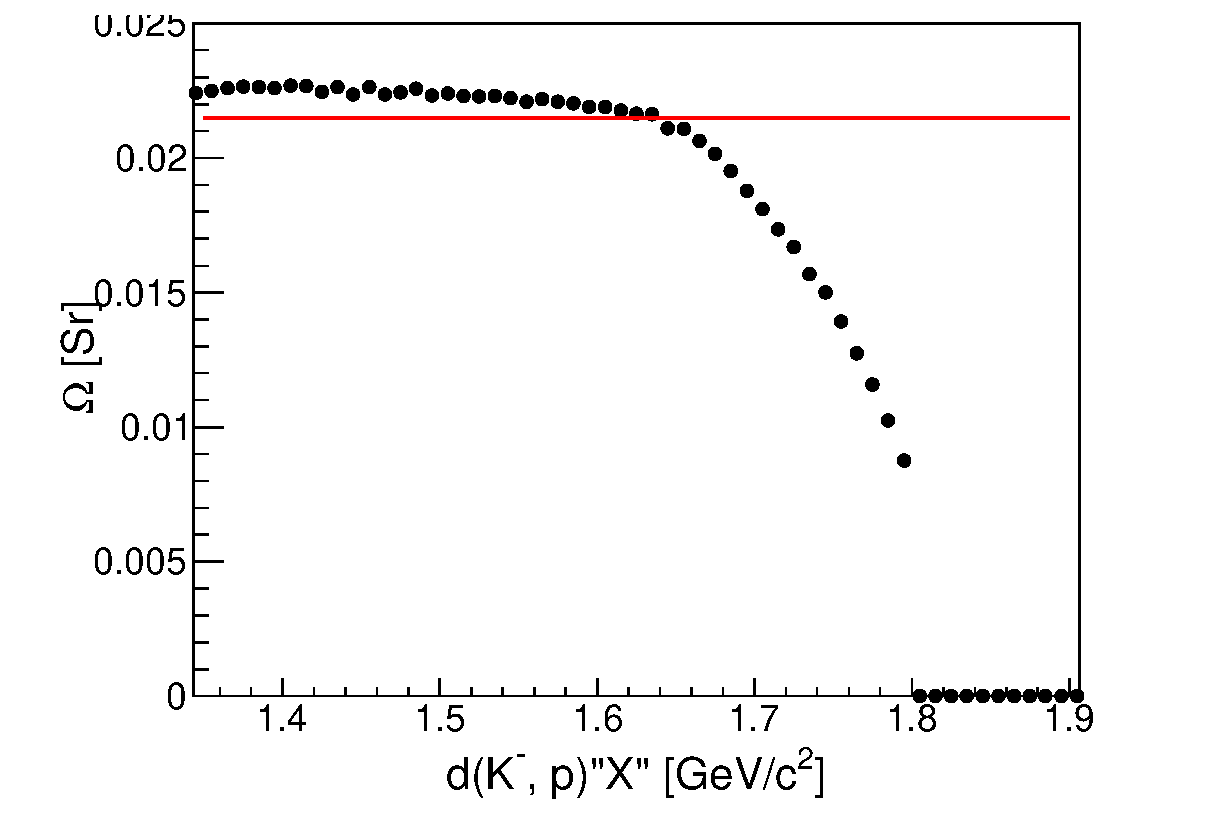
\includegraphics[width=8cm]{../pic/Run78/KP_ana/PCCVC_SA_1350_1900_no_npreac.eps}
  \caption{
    This figure indicates the solid angle of the forward detectors as function of the $d(K^-, p)$.
    Red line indicates the solid angle of the NC, which was calculated from the geometory.
  }
\end{figure}

In this subsection, forward scattered proton Monte Carlo simulation was explained.
The purposes of the MC sim are the solid angle estimation of the forward detectors for the forward scattered proton
and the CDS acceptance estimation for the $d(K^-, p)"\pi^-\Lambda$ and the $d(K^-, p)"\pi^-\Sigma^0"$.\\ 
Studies using the Monte Carlo simulation was used the Geant4 toolkit which simulates the motion and the reaction of various particles in any materials.
The detail setting and so on were described in Sec\ref{sec:geant4}.\\
First, the solid angle estimation was explained.
Because the inefficiency due to between the target and the PC/CVC was estimated before subsection, the reaction of a proton with other materials was cut except for the electromagnetic interaction. 
The forward emitted proton was generated only at the target fiducial volume and was injected the aperture of the Ushiwaka which adopted the calculated magnetic field map.
The $K^- d \rightarrow p_{forward} \Lambda \pi^-$ reaction was used for the study.
Events that can analyze the beamline and the CDS adopted as trigger events and events that can be identified as protons by forward detectors defined effective events.
The effective ratio of the each solid angle indicated at Fig\ref{fig:FC_SA}.
The solid angle of forward detectors was evaluated as the integral value of these 2D-histograms.
Because the bending angle depends on the field strength of the Ushiwaka magnet, this estimation was performed each bin of the $d(K^-, p)$.
The relation of the $d(K^-, p)$ and the solid angle was represented at Fig\ref{fig:FC_SA}
As described Sec\ref{sec:}, the solid angle was almost flat in the interested region. % To do sec:XXX

Next is about the CDS acceptance for the $d(K-, p)"\pi^-\Lambda"$ and the $d(K^-, p)"\pi^-\Sigma^0"$.
In this study, the physics reaction was used because the purpose of the	study is a realistic acceptance estimation of the CDS.
So, the same analysis procedure of the real data was adapted to the data generated by the MC sim and finally remaining events was defined as effective events.
Detector resolutions were determined to reproduce the well-known particle peaks, which was described as Sec\ref{sef:}. % To do sec:XXX
For this estimation, we simulate the following reactions\\
\begin{eqnarray}
  K^- d \rightarrow p_{forward} (\Lambda \pi^-)  \label{eq:KD_p_pimL}\\
  K^- d \rightarrow p_{forward} (\Sigma^0 \pi^-) \label{eq:KP_p_pimS0}
\end{eqnarray}
The $p_{forward}$ injected at a forward angle which is $\theta<8^{\circ}$ and the remaining $\pi^- Y$ mass using flat distribution between the $\pi\Sigma$ mass threshold to 1.8$GeV/c$.
In these, Events that can analyze the kaon beam and the forward proton were used trigger events for this estimation.
Estimated acceptance was indicated Fig\ref{fig:acc_kp}.

\begin{figure}[htbp]
  \centering
  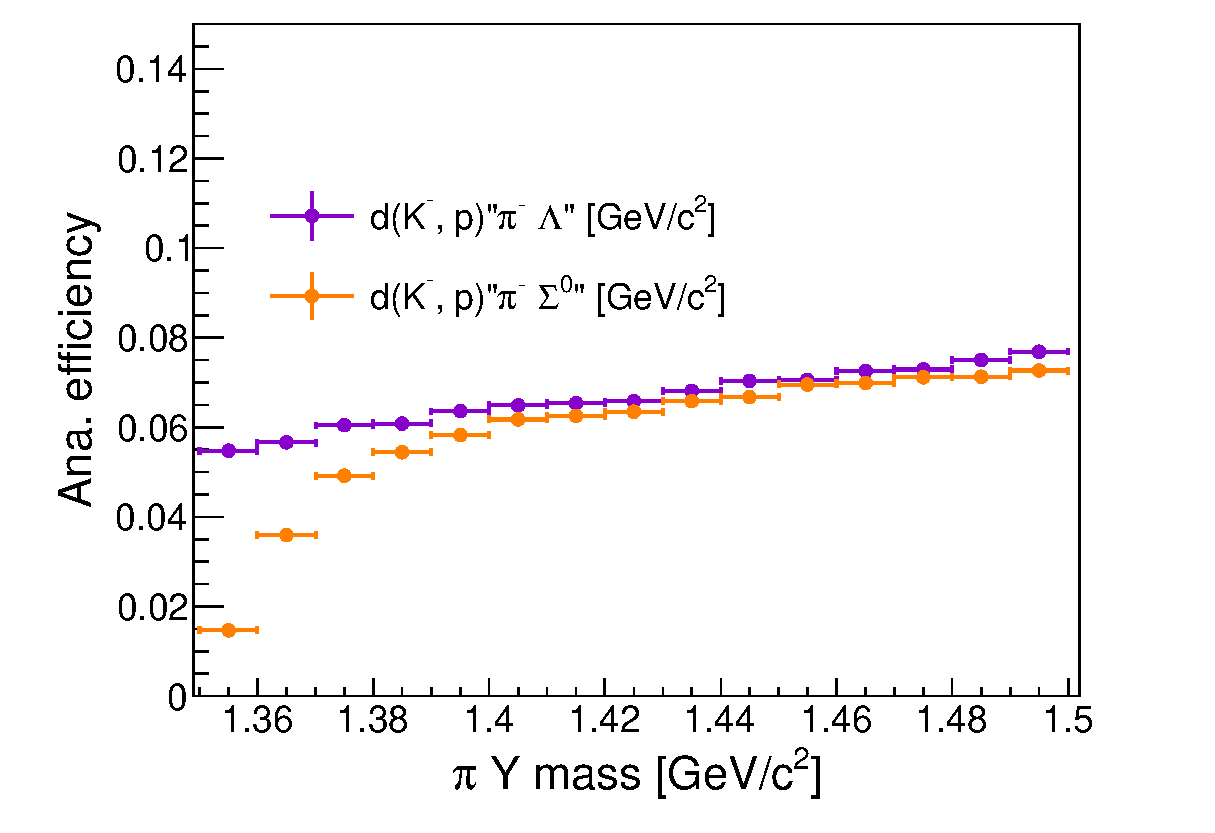
\includegraphics[width=8cm]{../pic/Run68/KP_ana/kp_acc.eps}
  \caption{
    This figure shows acceptanes of the $d(K^-, p)"\pi^-Sigma^0$ and the $d(K^-, p)"\pi^-\Lambda"$ which was estimated by the Monte Calro simulation.
  }
  \label{fig:acc_kp}
\end{figure}
